% Copyright 2020, Gernot Heiser
% SPDX-License-Identifier: CC-BY-SA-4.0

% Setting this to true turns on the ``draft'' watermark
\newif \ifDraft         \Draftfalse
%\Drafttrue

% Note: the draft option marks overfull lines but disables hyperlinks!
\documentclass[english,a4paper,12pt\ifDraft,draft\fi]{report}
%\documentclass[a4paper,11pt,titlepage]{article}
%\Drafttrue

\usepackage[]{sel4}
\typeout{After loading seL4}

%%% Hyperlinks embed links for references in the PDF output (both for
%%% internal as well as external links).
\newif \ifhyperlinks    \hyperlinkstrue
%%% When using this you should use \autoref{label} instead of
%%% Section~\ref{label}. This will make ``Section'' part of the link, not
%%% just the number.

\usepackage{xspace}             % to fix spacing in macros producing words. Eg:
\newcommand{\seLfour}{seL4\xspace} % use as normal text, examples below.

% Example of multi-letter symbols for math mode:
\newcommand{\myFunc}{\mathrm{myFunc}}
\newcommand{\myVar}{\mathit{diff}}

% Leave this in here, it is often useful to deal with latexdiff breakage.
% Put it around breakage-causing segments (in both versions to be diffed!)
\newenvironment{DIFnomarkup}{}{}

\usepackage{graphicx}
\setkeys{Gin}{keepaspectratio=true,clip=true,draft=false,width=\linewidth}
\graphicspath{{./imgs/}}
\usepackage{url,verbatim,datetime,tabularx}
\usepackage[olditem]{paralist}
\usepackage[authoryear]{natbib}

\ifx\undefined\chapter
  %\typeout{no chapters}
  \newcommand{\Sect}[1]{\section{#1}}
  \newcommand{\SSect}[1]{\subsection{#1}}
  \newcommand{\SSSect}[1]{\subsubsection*{#1}}
  \newcommand{\Acks}{\section*{Acknowledgments}}
\else
  %\typeout{have chapters}
  \newcommand{\Sect}[1]{\chapter{#1}}
  \newcommand{\SSect}[1]{\section{#1}}
  \newcommand{\SSSect}[1]{\subsection*{#1}}
  \newcommand{\Acks}{\chapter*{Acknowledgments}}
\fi

  \newcommand{\code}[1]{\texttt{#1}}

  \newcommand{\Break}{\ \nopagebreak\\}

  \newlength{\chillilng}\setlength{\chillilng}{8mm}
  \newlength{\chillimarg}\setlength{\chillimarg}{10mm}
  \newcommand{\chilli}{
\includegraphics[width=\chillilng]{chilli}}
  \newcommand{\chilliItem}{\raisebox{-5mm}[1ex][0pt]{%
      \makebox[\chillilng][r]{\chilli}}}
  \newcommand{\chilliSect}{\raisebox{-2mm}[1ex][0pt]{\chilli\hspace{0.8em}}}
  \newenvironment{Chilli}{
    \begin{list}{}{
      \setlength{\labelwidth}{\chillilng}
      \setlength{\leftmargin}{\chillimarg}}
    \item[\chilliItem]
    }
  {\end{list}}

\ifDraft
  \usepackage{draftwatermark}
  \SetWatermarkLightness{0.85}
  \newcommand{\Comment}[1]{\textbf{\textsl{#1}}}
  \newenvironment{LongComment}[1] % multi-paragraph comment, argument is owner
    {\begingroup\par\noindent\slshape \textbf{Begin Comment[#1]}\par}
    {\par\noindent\textbf{End Comment}\endgroup\par}
  \newcommand{\FIXME}[1]{\textbf{\textsl{FIXME: #1}}}
  \newcommand{\TODO}[1]{\textbf{\textsl{TODO: #1}}}
\else
  \newcommand{\Comment}[1]{\relax}
  \newenvironment{LongComment}[1]{\expandafter\comment}{\expandafter\endcomment}
  \newcommand{\FIXME}[1]{\relax}
  \newcommand{\TODO}[1]{\relax}
  \fi

  \newcommand{\gernot}[1]{\Comment{#1 \colorbox{yellow}{[gernot]}}}

  \hypersetup{pdftex,
                      pagebackref,
                      hyperindex,
                      bookmarks,
                      pdftitle={The seL4 Microkernel -- An Introduction},
                      pdfauthor={Gernot Heiser},
                      pdfsubject={seL4 Foundation Whitepaper Revision 1.2},
                      pdfkeywords={seL4, microkernel, performance},
                      pdfdisplaydoctitle=true}

\begin{document}

  %% Capitalisation of cross references
  \renewcommand{\chapterautorefname}{Chapter}
  \renewcommand{\sectionautorefname}{Section}
  \renewcommand{\subsectionautorefname}{Section}
  \renewcommand{\subsubsectionautorefname}{Section}
  \renewcommand{\appendixautorefname}{Appendix}
  \renewcommand{\Hfootnoteautorefname}{Footnote}
  %% Commands for index
  \newcommand{\Htextbf}[1]{\textbf{\hyperpage{#1}}}

  \renewcommand{\topfraction}{0.9}
  \renewcommand{\bottomfraction}{0.9}

  % \textsuperscript{\textregistered} doesn't produce the right result here
  \title{The seL4\raisebox{1ex}[0pt][0pt]{\large\textregistered} Microkernel}
  \subtitle{An Introduction}

  \author{Gernot Heiser}
%  \authortitle{Author's title}
  \email{gernot@sel4.systems}
  \docversion{Revision 1.2 of 2020-06-10}
  \date{}

  \thispagestyle{plain}
  \maketitle 
  \doCopyright[2020]

\begin{abstract}
    This whitepaper provides an introduction to and overview of
    seL4. We explain what seL4
    is (and is not) and explore its defining features. We explain what
    makes seL4
    uniquely qualified as the operating-system kernel of choice for
    security- and safety-critical systems, and generally embedded and
    cyber-physical systems. In particular, we explain
    seL4's assurance story, its security- and safety-relevant
    features, and its benchmark-setting performance. We also discuss
    typical usage scenarios, including incremental cyber retrofit of
    legacy systems.

    \vspace{6ex}
    \setcounter{page}{0}

    \newcommand{\Sub}{{\boldmath\(\rightarrow\)}\xspace}
    \textbf{CCS Concepts}
    \begin{compactitem}
    \item Software and its engineering \Sub Operating Systems
    \item Security and privacy \Sub Systems security
    \item Security and privacy \Sub Formal methods and theory of security
    \item Computer systems organization \Sub Real-time systems \Sub
      Real-time operating systems
    \item Computer systems organization \Sub Real-time systems \Sub
      Dependable and fault-tolerant systems and networks
    \end{compactitem}
    \vspace{2ex}

    \textbf{Keywords}\\
    seL4, microkernel, performance
    \vspace{2ex}

    \textbf{Reference Format:}\\
    Gernot Heiser. The seL4 Microkernel -- An Introduction. White
    paper. The seL4 Foundation, \thedocversion.
  \end{abstract}

%  \tableofcontents

%  \cleardoublepage

  \Sect{What Is seL4?}\label{s:intro}

  \begin{description}
  \item[seL4 is an operating system microkernel]\Break
    An \href{https://en.wikipedia.org/wiki/Operating_system}{operating
      system} (OS) is the low-level system software that controls a
    computer system's resources and enforces security. Unlike
    application software, the OS has
    exclusive access to a more privileged execution mode of the processor (\emph{kernel mode})
    that gives it direct access to hardware. Applications only ever
    execute in
    \emph{user mode} and can only access hardware as permitted by the
    OS.

    An OS
    \href{https://en.wikipedia.org/wiki/Microkernel}{microkernel} is a
    minimal core of an OS, reducing the code executing at higher
    privilege to a minimum. seL4 is a member of the
    \href{https://en.wikipedia.org/wiki/L4_microkernel_family}{L4
      family of microkernels} that goes back to the mid-1990s.
    (And no, \emph{seL4 has nothing to do with seLinux.})

  \item[seL4 is also a hypervisor] \Break
    seL4 supports virtual machines that can run a fully fledged guest OS
    such as Linux. Subject to seL4's enforcement of communication
    channels,  guests and their applications can communicate with
    each other as well as with native applications.

   Learn  more about what it means that seL4 is a microkernel and its use as
    a hypervisor in \autoref{s:ukernel}. And learn about real-world
    deployment scenarios, including approaches for retrofitting security into
    legacy systems in \autoref{s:retrofit}.

  \item[seL4 is proved correct]\Break
    seL4 comes with a formal, mathematical, machine-checked
    \emph{proof of implementation correctness}, meaning the kernel is
    in a very strong sense ``bug free'' with respect to its specification.
    In fact, seL4 is the world's
    first OS kernel with such a proof at the code level
    \citep{Klein_EHA_etal_09}.

  \item[seL4 is provably secure]\Break
    Besides implementation correctness, seL4 comes with further proofs of
    \emph{security enforcement} \citep{Klein_AEMSKH_14}. They say that
    in a correctly configured seL4-based system,  the kernel
    guarantees the classical security properties of
    \emph{confidentiality, integrity and availability}. More about
    these proofs in \autoref{s:proofs}.

  \item[seL4 improves security with fine-grained access control
    through capabilities]\Break
    \href{https://en.wikipedia.org/wiki/Capability-based_security}{Capabilities}
    are access tokens which support very fine-grained control over which
    entity can access a particular resource in a system. They support
    strong security according to the
    \href{https://en.wikipedia.org/wiki/Principle_of_least_privilege}{principle
      of least privilege} (also called principle of least authority,
    POLA). This is a core design principle of highly secure system,
    and is impossible to achieve with the way access control happens
    in mainstream systems such as Linux or Windows.

    seL4 is still the \emph{world's only OS that is both
      capability-based and formally verified}, and as such has a
    defensible claim of being the world's most secure OS. More about capabilities
    in \autoref{s:caps}.

  \item[seL4 ensures safety of time-critical systems] \Break% ~\nopagebreak\\
    seL4 is the world's only OS kernel (at least in the open
    literature) that has undergone a complete and sound analysis of
    its \emph{worst-case execution time} (WCET)
    \citep{Blackham_SCRH_11, Sewell_KH_17}. This means,
    if the kernel is configured appropriately, all kernel
    operations are bounded in time, and the bound is known. This is a
    prerequisite for building \emph{hard real-time systems}, where
    failure to react to an event within a strictly bounded time period
    is catastrophic.

  \item[seL4 is the world's most advanced mixed-criticality OS] \Break
    seL4 provides strong support for
    \href{https://en.wikipedia.org/wiki/Mixed_criticality}{mixed
      criticality real-time systems} (MCS), where the timeliness of critical
    activities must be ensured even if they co-exist with less trusted
    code executing on the same platform. seL4 achieves this with a
    flexible model that retains good resource utilisation, unlike the
    more established MCS OSes that use strict (and inflexible) time
    and space partitioning \citep{Lyons_MAH_18}. More on seL4's
    real-time and MCS support in \autoref{s:rtos}.

  \item[seL4 is the world's fastest microkernel] \Break
    Traditionally, systems are either (sort-of) secure, or they are
    fast. seL4 is unique in that it is both. seL4 is designed to
    support a wide range of
    real-world use cases, whether they are
    security- (or safety-)critical or not, and excellent performance
    is a requirement. More on seL4's
    performance in \autoref{s:perf}.

  \item[seL4 is pronounced ``ess-e-ell-four''] \Break
    The pronunciation ``sell-four'' is deprecated.
  \end{description}

  \SSSect{How to read this document}

  This document is meant to be approachable by a wide
  audience. However, for completeness, we will add some deeper
  technical detail in places.

  \begin{Chilli}
    Such detail will be marked with a chilli, like the one on the left. If you
    see this then you know you can safely skip the marked passage if
    you think the technical description is too ``spicy'' for your
    taste, or if you are simply not interested in this level of
    detail. Only other chillied passages will assume you have read it.
  \end{Chilli}

  \SSSect{\chilliSect Technical section}
  Where the chilli appears in a section title, such as here, this
  indicates that the whole section is fairly technical and can be skipped.

  \Sect{seL4 Is a Microkernel and a Hypervisor, It Is Not an
    OS}\label{s:ukernel}

  \SSect{Monolithic kernels vs microkernels}

  To understand the difference between a mainstream OS, such as Linux,
  and a microkernel, such as seL4, let's look at
  \autoref{f:osstruct}.

  \begin{figure}[hb]
    \centering
    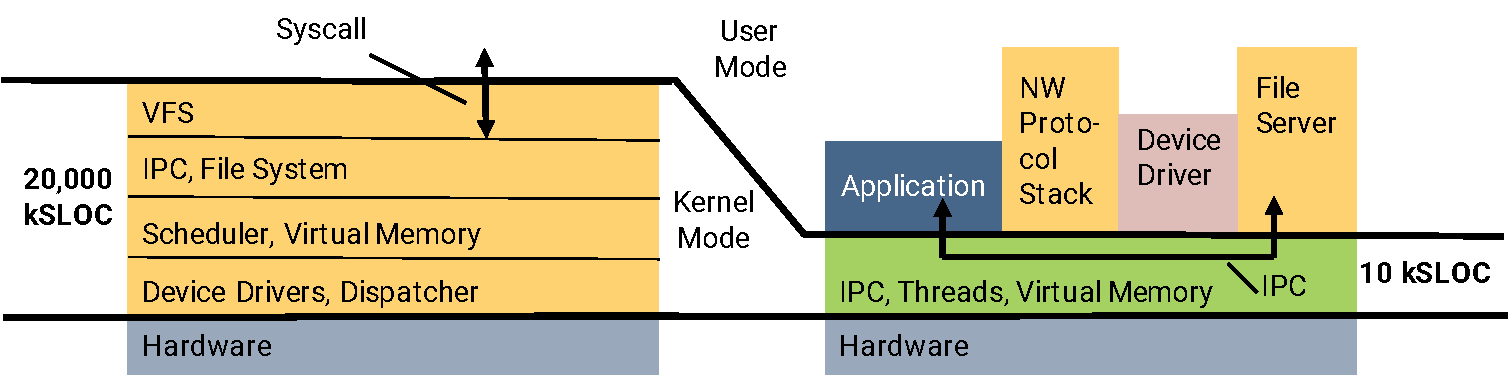
\includegraphics[width=1.0\textwidth]{kernel}
    \caption[Operating-system structure.]{Operating-system structure:
      Monolithic kernel (left) vs microkernel (right).}
    \label{f:osstruct}
  \end{figure}

  The left side presents a (fairly abstracted) view of the
  architecture of a system such as Linux. The yellow part is the OS
  \emph{kernel}, it offers services such as file storage and
  networking to applications.  All the code that implements those
  services executes in the \emph{privileged mode} of the hardware,
  also called \emph{kernel mode} or \emph{supervisor mode} --
  the execution mode that has unfettered access and control of all
  resources in the system. In contrast, applications run in
  unprivileged, or \emph{user mode}, and do not have direct access to
  many hardware resources, which must be accessed through the OS. The
  OS is internally structured in a number of layers, where each layer
  provides abstractions implemented by layers below.

  The problem with privileged-mode code is that it is dangerous: If
  anything goes wrong here, there's nothing to stop the damage. In
  particular, if this code has a bug that can be exploited by an
  attacker to run the attacker's code in privileged mode (called a
  privilege-escalation or arbitrary code-execution attack) then the
  attacker can do what they want with the system. Such flaws are the
  root problem of the many system compromises we experience in
  mainstream systems.

  Of course, software bugs are mostly a fact of life, and
  OSes are not different.  For example, the Linux kernel comprises of
  the order of 20 million lines of source code (20\,MSLOC); we can
  estimate that it contains literally tens of thousands of bugs
  \citep{Biggs_LH_18}. This is obviously a huge attack surface! This
  idea is captured by saying that Linux has a large \emph{trusted computing
    base} (TCB), which is defined as the subset of the overall system
  that must be trusted to operate correctly for the system to be
  secure.

  The idea behind a microkernel design is to drastically reduce the
  TCB and thus the
  attack surface. As schematically shown at the right of
  \autoref{f:osstruct}, the kernel, i.e.\ the part of the system
  executing in privileged mode, is much smaller. In a well-designed
  microkernel, such as seL4, it is of the order of ten thousand lines
  of source code (10\,kSLOC). This is literally three orders of
  magnitude smaller than the Linux kernel, and the attack surface shrinks
  accordingly (maybe more, as the density of bugs probably
  grows more than linearly with code size).

  Obviously, it is not possible to provide the same functionality, in
  terms of OS services, in such a small code base. In fact, the
  microkernel provides almost no services: it is just a thin wrapper
  around hardware, just enough to securely multiplex hardware
  resources. What the microkernel mostly provides is isolation,
  sandboxes in which programs can execute without interference from
  other programs. And, critically, it provides a \emph{protected
    procedure call} mechanism, for  historic reasons called
  \emph{IPC}. This allows one program to securely call a function in a
  different program, where the microkernel transports function inputs
  and outputs between the programs and, importantly, enforces
  interfaces: the ``remote'' (contained in a different sandbox)
  function can only be called at an exported entrypoint, and only by
  explicitly authorised clients (who have been given the appropriate
  capability, see \autoref{s:caps}).

  \begin{Chilli}
    For a deeper explanation of what seL4 IPC is and is not, I
    recommend reading my blog \href{https://microkerneldude.wordpress.com/2019/03/07/how-to-and-how-not-to-use-sel4-ipc/}{How to (and how not to) use seL4 IPC}.
  \end{Chilli}

  The microkernel system uses this approach to provide the services
  the monolithic OS implements in the kernel. In the microkernel
  world, these services are just programs, no different from applications,
  that run in their own sandboxes, and provide an IPC interface for
  applications to call. Should a server be compromised, that compromise is
  confined to the server, its sandbox protects the rest of the
  system. This is in stark contrast to the monolithic case, where a
  compromise of an OS service compromises the complete system.

  This effect can be quantified: Our recent study shows that of the
  known Linux compromises classified as \emph{critical}, i.e.\ most
  severe, 29\% would be fully eliminated by a microkernel design, and
  another 55\% would be mitigated enough to no longer qualify as
  critical \citep{Biggs_LH_18}.

  \SSect{seL4 Is a microkernel, not an OS}


  \begin{figure}[ht]
    \centering
    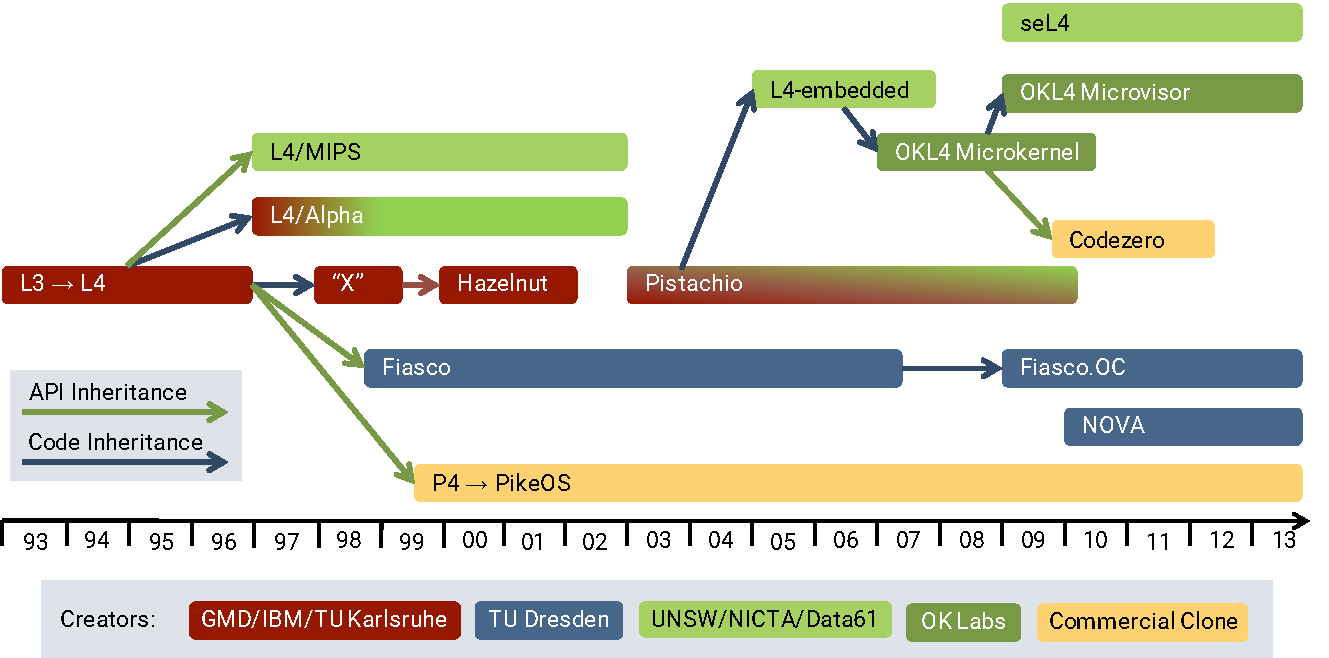
\includegraphics{l4family}
    \caption{L4 microkernel family tree.}
    \label{f:l4family}
  \end{figure}

  seL4 is a microkernel, and designed for generality while
  minimising the TCB. It is a member of the L4
  microkernel family, which goes back to the mid-'90s;
  \autoref{f:l4family} shows seL4's provenance. It was developed by our group at UNSW/NICTA,
  these days known as Trustworthy Systems (TS). At the time we
  had 15 years of experience in developing
  high-performance microkernels, and a track-record of
  real-world deployments: Our \emph{OKL4 Microkernel} shipped on
  billions of Qualcomm cellular modem chips, and our \emph{L4-embedded} kernel from the
  mid-Noughties runs on the secure enclave of all recent
  iOS devices (iPhones etc).

  Being a microkernel, seL4 contains none of the usual OS
  services; such services are  provided by  programs running in user
  mode. Besides the great advantages elaborated above,
  there are downsides to the microkernel design:  These components
  must come from somewhere. Some can be ported from open-source OSes, such as
  FreeBSD or Linux, or they can be written from scratch. But in any
  case, this is significant work.

  To scale up we need the help of the community, and the seL4
  Foundation is the key mechanism for enabling the community to
  cooperate and develop or port such services for seL4-based
  systems. The most important ones are device drivers, network
  protocol stacks, and file
  systems. \href{https://docs.sel4.systems/projects/available-user-components.html}{We
    have a fair number of these}, but much  more is needed.

  An important enabler is a component framework; it allows developers
  to focus on the code that implements the services, and automates
  much of the system integration. There are presently two main
  component frameworks for seL4, both open source: CAmkES and Genode.

  \href{https://trustworthy.systems/projects/TS/camkes/}{CAmkES} is a
  framework that is aimed at embedded and cyber-physical systems,
  which typically have a static architecture, meaning they consist of
  a defined set of components that does not change once the system has
  fully booted up.

  \href{https://genode.org/}{Genode} is in many ways a more powerful
  and general framework, that supports multiple microkernels and
  already comes with a wealth of services and device drivers,
  especially for x86 platforms. It is arguably more convenient
  to work with than CAmkES, and is certainly the way to get a
  complex system up quickly. However, Genode has drawbacks:
  \begin{inparaenum}
  \item As it supports multiple microkernels, not all as powerful as
    seL4, Genode is based on the least common denominator. In
    particular, it cannot use all of seL4's security and safety
    features.
  \item It has no assurance story. More on this in \autoref{s:camkes}.
  \end{inparaenum}

  \SSect{seL4 is also a hypervisor}\label{s:hyp}

  seL4 is a microkernel, but it is also a hypervisor: It is possible
  to run virtual machines on seL4, and inside the virtual machine (VM)
  a mainstream OS, such as Linux.

  \begin{figure}[ht]
    \centering
    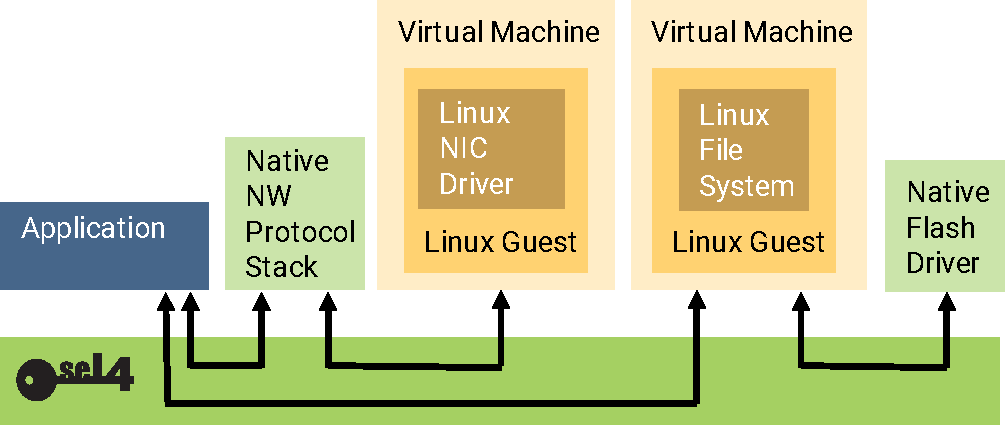
\includegraphics[width=0.9\textwidth]{hypervisor}
    \caption[VM-provided services]{Using virtualisation to integrate
      native OS services with Linux-provided services.}
    \label{f:vms}
  \end{figure}

  This enables an alternative way of provisioning system services, by
  having a Linux VM provide them. Such a setup is shown in
  \autoref{f:vms}, which shows how some services are borrowed from
  multiple Linux instances running as guest OSes in separate VMs.

  In this example, we provide two system services: networking and
  storage. Networking is provided by a native protocol stack
  running directly on seL4, lwIP or PicoTCP are frequently used
  stacks. Instead of porting a network driver, we borrow one from
  Linux, by running a VM with a stripped-down Linux guest that has
  little more than the NIC driver. The protocol stack communicates
  with Linux via an seL4-provided channel, and the application
  similarly obtains network services by communicating with the
  protocol stack. Note that in the setup shown in the figure, the
  application has no channel to the NIC-driver VM, and thus cannot
  communicate with it directly, only via the NW stack; this is enabled
  by seL4's capability-based protection (see \autoref{s:caps}).

  A similar setup is shown for the storage service; this time the
  file system is a Linux one running in a VM, while the storage
  driver is native. Again, communication between the components is
  limited to the minimum channels required. In particular, the app
  cannot talk to the storage driver (except through the file system),
  and the two Linux systems cannot communicate with each other.

  \begin{figure}[tb]
    \centering
    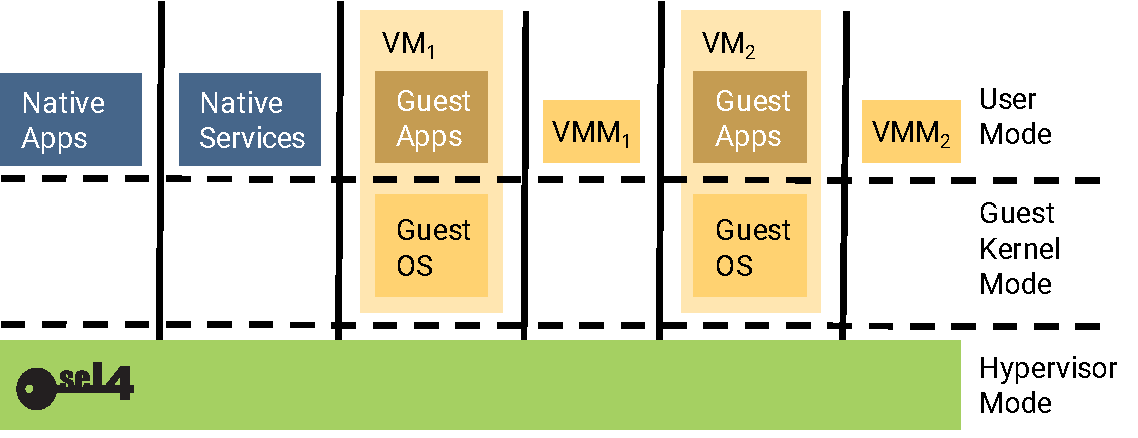
\includegraphics{vmm}
    \caption{seL4 virtualisation support with usermode VMMs.}
    \label{f:vmm}
  \end{figure}

  \begin{Chilli}
    When used as a hypervisor, seL4 runs in the appropriate hypervisor
    mode (EL2 on Arm, Root Ring-0 on x86, HS on RISC-V), which is a
    higher privilege level than the guest operating system. Just as
    when running as the OS kernel, it only does the minimum work
    that has to be performed in the privileged (hypervisor) mode and leaves everything
    else to user mode.

    Specifically this means that seL4 performs \emph{world switches},
    meaning it switches virtual machine state when a VM's execution
    time is up, or VMs must be switched for some other reason. It also
    catches virtualisation exceptions (``VM exits'' in Intel lingo)
    and forwards them to a user-level handler, called the
    \emph{virtual machine monitor} (VMM). The VMM is then responsible
    for performing any emulation operations needed.

    Each VM has its private copy of the VMM, isolated from the guest
    OS as well as from other VMs, as shown in \autoref{f:vmm}. This
    means that the VMM cannot break isolation, and is therefore not
    more trusted than the guest OS itself. In particular, this means
    that there is no need to verify the VMM, as that would not add
    real assurance as long as the guest OS, typically Linux, is not
    verified.
  \end{Chilli}

  \SSect{seL4 is not seLinux}

  Many people confuse seL4 with seLinux (probably because seL4 might be
  mistaken as a shorthand for the 4\(^\textrm{th}\) version of seLinux).
  Fact is that seL4 has nothing whatsoever to do with seLinux, other
  than both being open source. They share no code nor abstractions.   seLinux is
  not a microkernel, it is a security policy framework built into Linux. While in some ways
  more secure than standard Linux, seLinux suffers from the same
  problem as standard Linux:
  a huge TCB, and correspondingly huge attack surface. In other words,
  seLinux is an add-on to a fundamentally insecure operating system
  and thus remains fundamentally insecure. In contrast, seL4 provides
  bullet-proof isolation from the ground up.

  In short, seLinux is not suitable for truly security-critical uses,
  while seL4 is designed for them.

  \Sect{seL4's Verification Story}\label{s:proofs}

  In 2009, seL4 became the world's first OS kernel with a machine-checked
  functional correctness proof at the source-code level. This proof was 200,000
  lines of proof script at the time, one of the largest ever (we think it was
  the second largest then). It showed that a functionally correct OS kernel is
  possible, something that until then had been considered infeasible.

  Since then we have extended the scope of the verification to higher
  level properties, \autoref{f:proofs} shows the chain of proofs,
  which are explained below. Importantly, we maintained the proof with the
  ongoing evolution of the kernel: Commits to the mainline kernel
  source are only allowed if they do not break proofs, otherwise the poofs
  are updated as well. This \emph{proof engineering} is also a
  novelty. Our seL4 proofs constitute by
  far the largest proof base that is actively maintained. The set of proofs has by
  now grown to well over a million lines, most of this manually
  written and then machine checked.

  \begin{figure}[bh]
    \centering
    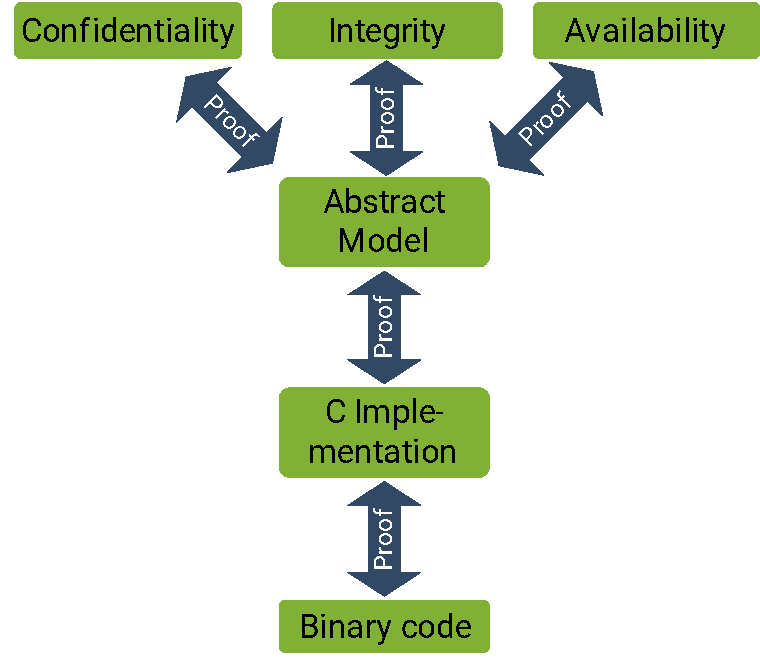
\includegraphics[width=0.6\textwidth]{proofs}
    \caption{seL4's proof chain.}
    \label{f:proofs}
  \end{figure}

  \SSect{Correctness and security enforcement}

  \SSSect{Functional correctness}

  The core of seL4's verification is the functional correctness proof, which says that the
  C implementation is free of implementation defects.
  More precisely, there is a formal
  specification of the kernel's functionality, expressed in a
  mathematical language called \emph{higher-order logic} (HOL). This
  is represented by the box labelled \emph{abstract model} in the
  figure. The functional correctness proof then says that the C
  implementation is a \emph{refinement} of the abstract model, meaning
  the possible behaviours of the C code are a subset of those allowed by the
  abstract model.


  \begin{Chilli}
    This informal description glosses over a lot of detail. Here is some
    of it in case you wonder.

    C is not a formal language; in order to allow reasoning about a C
    program in the theorem prover (we use Isabelle/HOL), it has to be
    transformed into mathematical logic (HOL). This is done by a C
    parser written in Isabelle. The parser defines the semantics of
    the C program, and gives it meaning in HOL according to this semantics.
    It is this formalisation
    which we prove to be a refinement of the mathematical (abstract) model.

    Note that C does not have an official mathematical semantics, and
    parts of the C language are notoriously subtle and not necessarily
    that well defined. We solve this by restricting our use of C to a
    well-defined subset of the language, for which we have an
    unambiguous semantics. However, this does not guarantee that our
    assumed semantics for that subset is the same as the
    compiler's. More on that below.
  \end{Chilli}

  The  proof means that everything we want to
  know about the kernel's behaviour (other than timing) is expressed
  by the abstract spec, and the kernel cannot behave in ways that are
  not allowed by the spec. Among others, this rules out the usual
  attacks against operating systems, such as stack smashing,
  null-pointer dereference, any code injection or control-flow highjacking etc.

  \SSSect{Translation validation}

  Having a bug-free C implementation of the kernel is great, but still
  leaves us at the mercy of the C compiler. Those compilers (we use
  GCC) are themselves large, complex programs that have
  bugs. So we could have a bug-free kernel that gets compiled into a
  buggy binary.

  \begin{figure}[th]
    \centering
    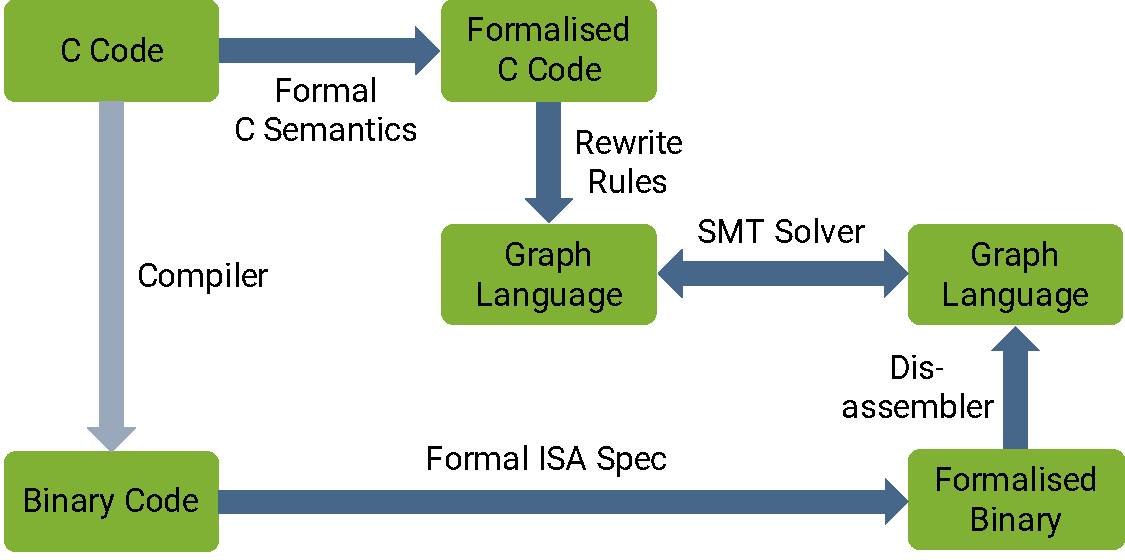
\includegraphics[width=0.85\textwidth]{binary}
    \caption{Translation validation proof chain.}
    \label{f:binary}
  \end{figure}

  In the security-critical space, compiler bugs are not the only
  problem. A compiler could be outright malicious, containing a Trojan
  that automatically builds in a back door when compiling the OS. The
  Trojan can be extended to automatically add itself when compiling
  the compiler, making it almost impossible to detect, even if the
  compiler is open-source! Ken Thompson explained this attack
  in his Turing Award lecture~\citep{Thompson_84}.

  To protect against defective or malicious compilers, we additionally
  verify the  executable binary that is produced by the compiler and
  linker. Specifically, we prove that the binary is a correct translation of the
  (proved correct) C code, and thus that the binary refines the
  abstract spec.

  \begin{Chilli}
    Unlike the verification of the C code, this proof is not done
    manually but by an automatic tool chain. It consists of several
    phases, as shown in \autoref{f:binary}. A formal model of the processor's instruction set
    architecture (ISA) formalises the binary in the theorem prover; we
    use an L3 formalisation of the RISC-V ISA, as well as the
    extensively tested L3 Arm ISA formalisation of \citet{Fox_Myreen_10}.

    Then a disassembler, written in the HOL4 theorem prover,
    translates this low-level representation into a higher-level
    representation in a graph language that basically represents
    control flow. This transformation is provably correct.

    The formalised C program is translated into the same graph
    language, through provably correct transformations in the Isabelle/HOL theorem
    prover. We then have two programs, in the same representation,
    which we need to show equivalent. This is a bit
    tricky, as compilers apply a number of heuristic-driven
    transformations to optimise the code. We apply a number of such
    transformations through rewrite rules on the graph-language
    representation of the C program (still in the theorem prover, and
    thus provably correct).

    In the end we then have two programs that are quite similar but
    not the same, and we need to prove that they have the same
    semantics. In theory this is equivalent to the halting problem
    and as such unsolvable. In practice, what the compiler does is
    deterministic enough to make the problem tractable. We do this by
    throwing the programs, in small chunks, at multiple \href{https://en.wikipedia.org/wiki/Satisfiability_modulo_theories}{SMT solvers}. If one of these can
    prove that all the corresponding pieces have the same semantics,
    then we know that the two programs are equivalent.

    Note also that the C program that is proved to refine the abstract
    spec, and the C program that we prove to be equivalent to the
    binary, are the same Isabelle/HOL formalisations. This means that
    our assumptions on C semantics drop out of the assumptions made by
    the proofs. Altogether, the proofs
    not only show that the compiler did not introduce bugs, but also
    that its semantics for the C subset we use are the same as ours.
  \end{Chilli}

  \SSSect{Security properties}

  \autoref{f:proofs} also shows proofs between the abstract spec and
  the high-level security properties \emph{confidentiality},
  \emph{integrity} and \emph{availability} (these are commonly
  dubbed the \emph{CIA properties}). These  state that the
  abstract spec is actually useful for security: They prove that in a
  correctly configured system, the kernel will enforce these
  properties.

  Specifically, seL4 enforces
  \begin{description}
  \item[confidentiality:] seL4 will not allow an entity to read (or
    otherwise infer) data without having been explicitly given read access
    to the data;
  \item[integrity:] seL4 will not allow an entity to modify data
    without having been explicitly given write access to the data;
  \item[availability:] seL4 will not allow an entity to prevent another
    entity's authorised use of resources.
  \end{description}

  \begin{Chilli}
    These proofs presently do not capture properties associated with
    time. Our confidentiality proofs rule out \emph{covert storage
      channels} but presently not \emph{covert timing channels}, which
    are used by such attacks as Spectre. Preventing timing channels
    is something we are working on
    \citep{Heiser_KM_19}. Similarly, the integrity and availability
    proofs presently do not cover timeliness, but our new MCS model
    \citep{Lyons_MAH_18} is designed to cover those aspects (see \autoref{s:mcs}).
  \end{Chilli}


  \SSSect{Proof assumptions}

  All reasoning about correctness is based on assumptions,
  whether the reasoning is formal, as with seL4, or informal, when
  someone thinks about why their program might be ``correct''. Every
  program executes in some context, and its correct behaviour
  inevitably depends on some assumptions about this context.

  One of the advantages of machine-checked formal reasoning is that it
  forces people to make those assumptions explicit. It is not possible
  to make unstated assumptions, the proofs will just not succeed if
  they depend on assumptions that are not clearly stated. In that
  sense, formal reasoning protects against forgetting assumptions, or
  not being clear about them; that in itself is a significant benefit
  of verification.

  The verification of seL4 makes three assumptions:
  \begin{description}
  \item[Hardware behaves as expected.] This should be obvious. The
    kernel is at the mercy of the underlying hardware, and if the
    hardware is buggy (or worse, has Trojans), then all bets are off,
    whether you are running verified seL4 or any unverified
    OS. Verifying hardware is outside the scope of seL4 (and
    the competency of TS); other people are working on that.
  \item[The spec matches expectations.] This is a difficult one,
    because one can never be sure that a formal specification means
    what we think it should mean. Of course, the same problem exists
    if there is \emph{no} formal specification: if the spec is informal or
    non-existent, then it is obviously impossible to precisely reason
    about correct behaviour.

    One can reduce this risk by proving properties about the spec, as
    we have done with our security proofs, which show that seL4 is
    able to enforce certain security properties. That then shifts the
    problem to the specification of those properties. They are much
    simpler than the kernel spec, reducing the risk of misunderstanding.

    But in the end, there is always a gap between the world of mathematics  and
    the physical world, and no end of reasoning (formal or informal)
    can remove this completely. The advantage of formal reasoning is
    that you know exactly what this gap is.
  \item[The theorem prover is correct.] This sounds like a serious
    problem, given that theorem provers are themselves large and
    complex programs. However, in reality this is the least concerning
    of the three assumptions. The reason is that the Isabelle/HOL
    theorem prover has a small core (of a few 10\,kSLOC) that checks
    all proofs against the axioms of the logic. And this core has
    checked many proofs small and large from a wide field of formal
    reasoning, so the chance of it containing a correctness-critical
    bug is extremely small.
  \end{description}

  \SSSect{Proof status and coverage}

  seL4 has been or is being verified for multiple architectures: Arm,
  x86 and RISC-V. Some of these are more complete than others, but the
  missing bits are generally worked on or waiting for funding. Please
  refer to the
  \href{https://docs.sel4.systems/projects/sel4/status.html}{seL4
    project status page} for details.

  \SSect{The CAmkES component framework}\label{s:camkes}

  \begin{figure}[b]
    \centering
    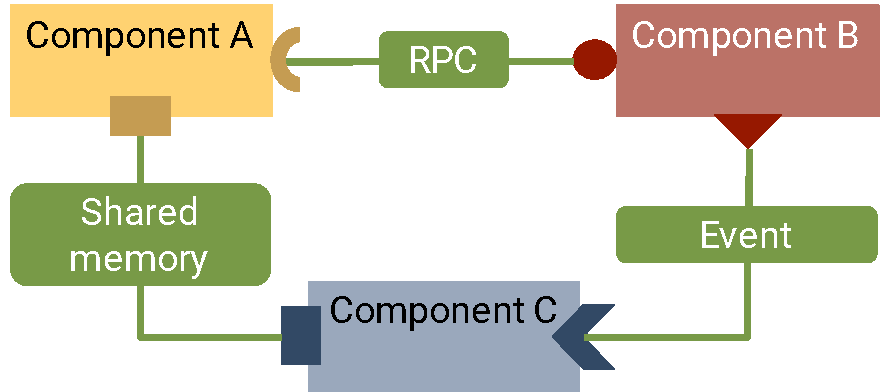
\includegraphics[width=0.6\textwidth]{camkes}
    \caption{CAmkES components and connectors.}
    \label{f:camkes}
  \end{figure}

  \href{https://trustworthy.systems/projects/TS/camkes/trustcomp.pml}{CAmkES}
  is a component framework that allows you to reason about a
  system architecturally, i.e.\ as a collection of sandboxed
  components with defined communication channels. \autoref{f:camkes}
  shows the main abstractions.
  \begin{description}
  \item[Components] are represented as square boxes. They represent
     programs, code and data, encapsulated by seL4.
  \item[Interfaces] are shown as decorations on the components. They
    define how a component can be invoked, or can invoke others. An
    interface is either imported (invoking an interface of another
    component) or exported (able to be invoked by another component's
    imported interface), except for the shared-memory interface, which
    is symmetric.
  \item[Connectors] connect like interfaces by linking an importing with an
    exporting interface. Connectors in CAmkES are always one-to-one,
    but broadcast or multicast functionality can be implemented on top
    of this model by building components that copy inputs to multiple outputs.
  \end{description}

  The CAmkES system is specified in a formal \emph{architecture
    description language} (the CAmkES ADL), which contains a precise
  description of the components, their interfaces and the connectors
  that link them up. The CAmkES promise to the system designer is
  that what is specified in the ADL (and visualised as in
  \autoref{f:camkes}) is a faithful representation of the possible
  interactions. In particular, it promises that no interactions are
  possible beyond those shown in the diagram.

  \begin{figure}[hb]
    \centering
    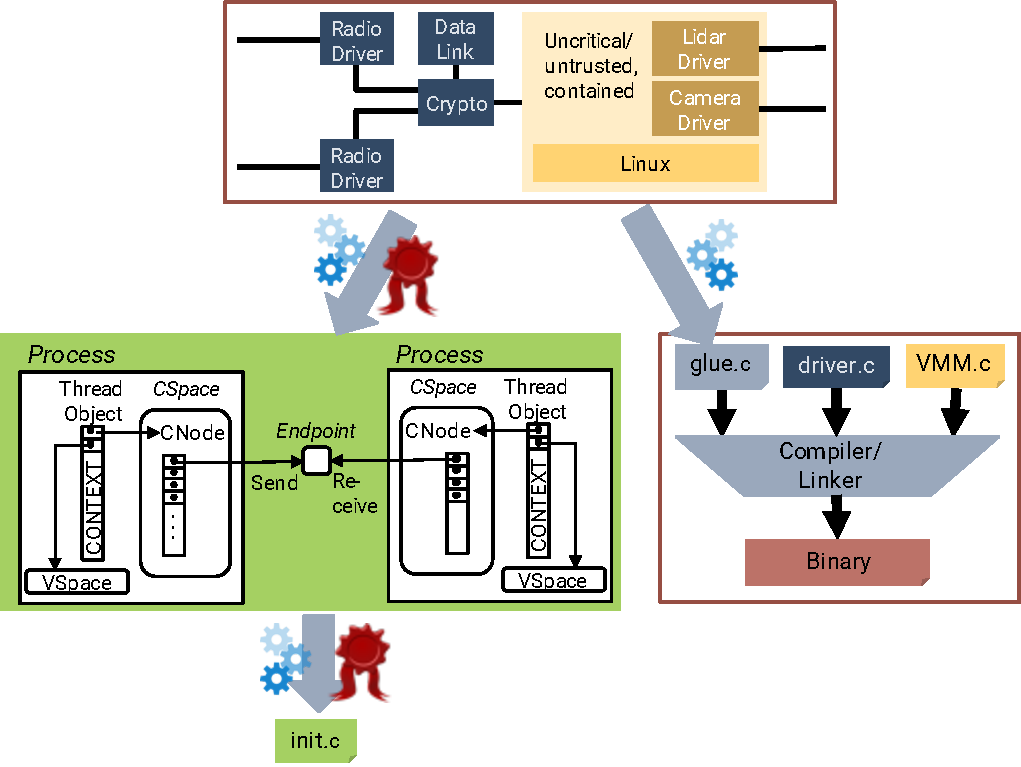
\includegraphics[width=\textwidth]{capdl}
    \caption{Verified architecture mapping and system generation
      (note that not all verification steps are of full strength
      yet). Green boxes are generated provably correct.}
    \label{f:capdl}
  \end{figure}

  Of course, this promise depends on enforcement by seL4, and the ADL
  representation must be mapped onto low-level seL4 objects and access
  rights to them. This is what the CAmkES machinery achieves, and is
  shown in \autoref{f:capdl}.

  In the figure, the architecture (i.e.\ what is described in the ADL)
  is shown at the top. This is a fairly simple system, consisting of
  four native components and one component that houses a virtual
  machine hosting a Linux guest with a couple of networking
  drivers. The Linux VM is only connected to other components via the
  crypto component, which ensures that it can only access encrypted
  links and cannot leak data.

  Even this simple system maps to hundreds if not thousands of seL4
  objects, an indication of the complexity reduction provided by the
  CAmkES component abstraction.

  For the seL4-level description we have another formal language,
  called CapDL (capability distribution language). The system designer
  never needs to deal with CapDL, it is a purely internal
  representation. The CAmkES framework contains a compiler which
  automatically translates CAmkES ADL into CapDL, indicated by the box
  arrow pointing left-down. The box in the left of the figure gives a
  (simplified) representation of the seL4 objects described in
  CapDL. (It is actually a simplified representation of a much simpler
  system, basically just the two components at the top of
  \autoref{f:camkes} and the connector between them.)

  The CapDL spec is a precise representation of access rights in the
  system, and it is what seL4 enforces. Which means that once the
  system gets into the state described by the CapDL spec, it is
  guaranteed to behave as described by the CAmkES ADL spec, and
  therefore the architecture-level description is sufficient for
  further reasoning about security properties.

  So we need assurance that the system boots up into the state
  described by the CapDL spec. We achieve this with a second
  automated step: We generate from CapDL the startup code that, as
  soon as seL4 itself has booted, takes control and generates all the
  seL4 objects referenced by the spec, including the ones describing
  active components, and distributes the \emph{capabilities} (see
  \autoref{s:caps}) that   grant access to those objects according to
  the spec. At the end of the execution of this init code, the system is
  provably in the state described by the CapDL spec, and thus in the
  state represented by the ADL spec.

  The third thing that gets generated from the ADL spec is the
  ``glue'' code between components. Sending data through a
  connector requires invocation of seL4 system calls, the exact
  details of which are hidden by the CAmkES abstraction. The glue code
  is   setting up these system  calls. For example, an ``RPC''
  connector abstracts the invocation of a function provided by another
  component as a regular function call performed by the client
  component.
\iffalse
  The glue-code generation is also verified, to guarantee
  that the invocation across component boundaries is functionally
  equivalent to executing the function's code (and using its state)
  inside the client component (while enforcing the module interface).
\fi

  \textbf{Note:} At the time of writing, the proofs about CAmkES and
  CapDL are not yet complete, but completion should not be far off.

  \begin{Chilli}
    Note also that none of the verification work mentioned deals with
    information leakage through timing channels (yet). This is a
    major unsolved research problem, but we're at the forefront of
    solving it.
  \end{Chilli}


  \Sect{About Capabilities}\label{s:caps}

  We encountered capabilities in \autoref{s:intro}, noting that they are
  access tokens. We will now look at the concept in more detail.

  \SSect{What are capabilities?}

  \begin{figure}[ht]
    \centering
    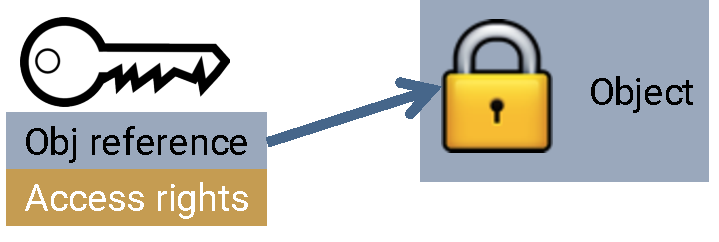
\includegraphics[width=0.5\textwidth]{cap}
    \caption[Capabilities are keys to objects]{A capability is key
      that conveys specific rights to a particular object.}
    \label{f:cap}
  \end{figure}

  As shown in \autoref{f:cap}, a capability is an object reference; in
  that sense it is similar to a pointer (and implementation of
  capabilities are often referred as ``fat pointers''). They are
  immutable pointers, in the sense that a capability will always
  reference the \emph{same} object, so each capability uniquely
  specifies a particular object.

  In addition to pointers, a capability also encodes access rights, in
  fact, the capability is an encapsulation of an object reference and
  the rights it conveys to that object. In a capability-based system,
  such as seL4, invoking a capability is the one and only way of
  performing an operation on a system object.

  For example, an operation may be to call a function in a
  component. The object reference embedded in the capability then
  points to an interface to that object, and conveys the right to
  invoke that function (i.e.\ a particular method on the component
  object). The capability may or may not at the same time
  convey the right to pass another capability along as a function
  argument (delegating to the component the right to use the object
  referenced by the capability argument).

  \begin{Chilli}
    This is a high-level description of what happens at the CAmkES
    abstraction level. In fact, at the CAmkES level, the capabilities
    themselves are abstracted away.

    Underneath, the connector is represented by an
    \emph{endpoint} object, and the client component needs a
    capability with \code{call} right.
  \end{Chilli}

  It is this fine-grained, object-oriented nature that makes
  capabilities the access-control mechanism of choice for
  security-oriented systems. The rights given to a component can be
  restricted to the absolute minimum it needs to do its job, as
  required by the
  \href{https://en.wikipedia.org/wiki/Principle_of_least_privilege}{principle
    of least privilege}.

  \begin{Chilli}
    Note that this notion of \emph{object capabilities} is quite
    different from (and far more powerful than) what Linux calls
    ``capabilities'', which are really access-control lists (ACLs) with
    system-call granularity. Linux capabilities, like all ACL
    schemes, suffer from the
    \href{https://en.wikipedia.org/wiki/Confused_deputy_problem}{confused
      deputy problem}, which is at the root of many security
    breaches, and explained in the next section. seL4 capabilities do not have this problem.
  \end{Chilli}

  \begin{Chilli}
    seL4 capabilities are also not susceptible to the attack of
    \citet{Boebert_84}; this attack applies to capabilities directly
    implemented in hardware while seL4's capabilities are
    implemented and protected by the kernel.
  \end{Chilli}

  \begin{Chilli}
    There are ten types of seL4 objects, all referenced by capabilities:
    \begin{description}
    \item[Endpoints] are used to perform protected function
      calls;
    \item[Reply Objects] represent a return path from a protected
      procedure call;
    \item[Address Spaces] provide the sandboxes around
      components (thin wrappers abstracting hardware page tables);
    \item[Cnodes] store capabilities representing a
      component's access rights;
    \item[Thread Control Blocks] represent threads of execution;
    \item[Scheduling Contexts] represent the right to access a
      certain fraction of execution time on a core;
    \item[Notifications] are synchronisation objects (similar
      to semaphores);
    \item[Frames]  represent physical memory that can be mapped
      into address spaces;
    \item[Interrupt objects] provide access to interrupt handling;  and
    \item[Untypeds] unused (free) physical memory
      that can be converted (``retyped'') into any of the other types.
    \end{description}
  \end{Chilli}

  \SSect{Why Capabilities}

  \SSSect{Fine-grained access control}

  As observed above, capabilities provide fine-grained access control,
  in line with the security principle of least privilege (also called
  \emph{principle of least authority}, short POLA). This is in contrast to
  the more traditional access-control model of access-control lists
  (ACLs), which are used in mainstream systems such as Linux or
  Windows, but also in commercial, supposedly secure systems, such as
  INTEGRITY or PikeOS.

  To understand the difference, consider how access control works in
  Linux: A file (and the file model applies to most other Linux
  objects) has an associated set of access-mode bits. Some of these
  bits determine what operations its owner can perform on the file,
  others represent the operations permitted for each member of the file's
  ``group'', and a final set gives default rights to everyone
  else. This is a subject-oriented scheme: It is a property of the
  subject (the process that is attempting access) that determines the
  validity of the access, and all subjects with the same value of the
  property (user ID or group ID) have the same rights. Moreover, these
  subjects have the same rights to \emph{all} files with the same
  settings of the access properties.

  This is a very coarse-grain form of access control, and is a
  fundamental limitation on what security policies can be enforced. A
  typical scenario is that a user wants to run an untrusted program
  (downloaded from the internet) to process a particular file but
  wants to prevent the program from accessing any other files the user
  has access. This is called a \emph{confinement} scenario, and there
  is no clean way to do this in Linux, which is the reason people came
  up with heavyweight workarounds (I like to call them hacks) such as
  ``chroot jails'', containers etc.

  With capabilities, this problem is straightforward to solve, as
  capabilities provide an object-oriented form of access
  control. Specifically, the kernel will allow an operation to go
  ahead if and only if the subject that requests the operation
  presents a capability that empowers it to perform the operation. In the
  confinement scenario, the untrusted app can only access files to
  which it has been given a capability. So Alice invokes the
  program, handing it a capability to the one file the program is
  allowed to read, plus a capability to a file where the
  program can write its output, and the program is unable to access
  anything else -- proper least privilege.

  \SSSect{Interposition and delegation}

  Capabilities have further nice properties. One is the ability to
  interpose access, which is a consequence of the fact that they are
  opaque object references. If Alice is given a capability to an
  object, she has no way of knowing what that object really is, all
  she can do is invoke methods on the object.

  For example, the system designer may pretend that the capability
  given to Alice refers to a file, when in fact it refers to a
  communication channel to a security monitor, which in turns holds
  the actual file capability. The monitor can examine Alice's
  requested operations and, if valid, performs them on the file on her
  behalf, while ignoring invalid ones. The monitor effectively
  virtualises the file.

  \begin{Chilli}
    Interposition has applications beyond enforcing security policies; the approach can
    be used for packet filtering, information-flow tracing and many
    more. A debugger can transparently interpose and virtualise object
    invokations. It can even be used to create objects lazily: Instead
    of an object reference, Alice is given a capability to a
    constructor, which then replaces the capability once the object has
    been created.
  \end{Chilli}

  Another advantage of capabilities is that they support safe and
  efficient delegation of privilege. If Alice wants to give Bob access
  to one of her objects, she can create (``mint'' in seL4 speak) a new
  capability to the object and hand it to Bob. Bob then can use that
  capability to operate on the object without referring back to
  Alice. (If, instead, Alice does want to stay in the loop, it can use
  virtualisation as explained above.)

  The new capability can have diminished rights; Alice can use this to
  give Bob only read-only access to the file. And Alice can revoke
  Bob's access at any time by destroying the derived capability she
  handed to Bob.

  Delegation is powerful and cannot easily and safely be done in ACL
  systems. A typical case of its use is setting up sub-systems that
  manage resources autonomously. When the system starts up, the
  initial process holds authority to all resources in the system
  (other than the small and fixed amount the kernel uses itself). This
  initial resource manager can then partition the system, by creating
  new processes (secondary resource managers) and handing them
  privilege to disjoint subsets of the system resources.

  The subsystems can then autonomously (without referring back to the
  original manager) control their subset of resources, while unable
  to interfere with each other. Only if they want to change the original
  resource allocation do they need to involve the original manager.

  \SSSect{\chilliSect Ambient authority and the confused deputy}

  \begin{figure}[th]
    \centering
    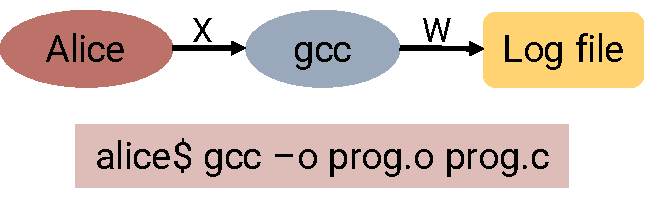
\includegraphics[width=0.45\textwidth]{deputy}
    \caption{The compiler as a confused deputy.}
    \label{f:deputy}
  \end{figure}

  ACLs have an unsolvable problem, generally called the \emph{confused
  deputy}. Let's look at a C compiler. It takes a C source file and
  produces an object-code output file, the file names are passed as
  arguments. To run the compiler, a user, Alice, must have execute
  permission on the compiler, as shown in \autoref{f:deputy}.

  Assume the compiler also creates an entry in a system-wide log file
  for auditing purposes. The log file is not accessible to normal
  users, so the compiler must execute with elevated privilege in order
  to write to the log file (traditionally done by making it a
  \emph{setuid} program).

  If Alice is malicious, she can trick the compiler into doing things
  it shouldn't do. For example, Alice can specify the password file as
  the output file when invoking the compiler. The compiler, unless it
  is written very carefully to avoid any potential abuse, will just
  open the output file (password file) and overwrite it with the
  compiled object code. It doesn't take a lot of skill for Alice to
  write a program which compiles such that the newly generated
  password file will give her privileges she should not have.

  The fundamental problem here is that ACL-based systems use
  \emph{ambient authority} for determining access rights. When the
  compiler opens its output file for writing, the OS determines the
  validity of the access by looking at the compiler's subject ID, to
  determine whether it has access to the object. It is up to the
  compiler to determine whether the operation is valid or not, making
  the compiler part of the system's TCB, meaning it has to be fully
  trusted to do the right thing under all circumstances.

  ACL-based systems can employ a number of workarounds to mitigate the
  particular problem here, for example, ensuring that the password
  file and the log file are in different security domains (which will
  not stop Alice from clobbering the log file, which in itself is a
  useful thing to do for an attacker covering her traces). This then
  sets up the usual arms race of attacks and workarounds, which is
  always a losing proposition for the good guys.

  The confusion arises due to ambient authority: The validity of
  an operation is determined by the security state of the agent
  (compiler), which in this case is a deputy operating on behalf of an
  original agent (Alice). For proper security, the access must be
  determined by Alice's security state. This means that denomination
  (the reference to the file) and authority (the right to perform
  operations on the file) must be coupled, a principle called \emph{no
    designation without authority}. If that is the case, then the
  compiler invokes the designated object (output file) with the
  authority that comes with the designation (from Alice), and Alice
  can no longer confuse the deputy.

  This is exactly what a capability system enforces. In such a system,
  Alice needs to hold three capabilities: an execute capability on the
  compiler, a read capability on the input file, and a write
  capability on the output file. She invokes the compiler with the
  execute capability and passes the other two as arguments. When the
  compiler then opens the output file, it does so with the capability
  provided by Alice, and there is no more confusion possible. The
  compiler uses a separate capability, which it holds itself, for
  opening the log file, keeping the two files well separated. In
  particular, it is impossible for Alice to trick the compiler into
  writing to a file she has no access to herself.

  The confused deputy problem is the ``killer app'' for capabilities,
  as the problem is unsolvable with ACLs. Hence, next time someone is
  trying to sell you a ``secure'' OS, not only ask whether they have
  a correctness proof for the OS, but also whether it uses
  capability-based access control. If the answer to either questions
  is ``no'', then you're being offered snake oil.

  \Sect{Support for Hard Real-Time Systems}\label{s:rtos}

  seL4 is designed as a protected-mode real-time OS. This means that
  unlike classical RTOSes, seL4 combines real-time capability with
  memory protection, for security as well as part of its support for
  mixed-criticality systems.

  \SSect{General real-time support}

  seL4 has a simple, priority-based scheduling policy that is easy to
  understand and analyse, a core requirement for hard real-time
  systems. The kernel will, on its own, never adjust priorities, so
  the user is in control.

  Another requirement are bounded interrupt latencies. seL4, like most
  members of the L4 microkernel family, executes with interrupts
  disabled while in kernel mode. This design decision greatly
  simplifies the kernel design and implementation, as the kernel (on a
  unicore processor) requires no concurrency control. seL4's formal
  verification would otherwise be infeasible, but the design is also
  an enabler for excellent average-case performance.

  \begin{Chilli}
    There is a widespread belief that a real-time OS must be
    preemptible, except for short critical sections, in order to keep
    interrupt latencies low. While true for traditional unprotected
    RTOSes running on simple microcontrollers, this belief is mistaken
    for a protected-mode system, such as seL4. The reason is that when
    running on a powerful microprocessor with memory protection
    enabled, the time for entering the kernel, switching context, and
    exiting the kernel, is significant, and not much less than a seL4
    system call. In terms of interrupt latencies, little could be
    gained by a preemptible design, but the cost in terms of
    complexity would be very high, making a preemptible design
    unjustified.
  \end{Chilli}

  This works as long as all system calls are short. In seL4 they
  generally are, but there are exceptions. Especially revoking a
  capability can be a long-running operation. seL4 deals with this
  situation by breaking such operations into short sub-operations, and
  making it possible to abort and restart the complete operation after
  each sub-operation, should there be a pending interrupt.

  \begin{Chilli}
    The approach is called incremental consistency. Each sub-operation
    transforms the kernel from a consistent state into another
    consistent state. The operation is structured such that after
    aborting, the operation can be restarted without repeating the
    sub-operations that had succeeded before the abort. The kernel
    checks for pending interrupts after each sub-operation. If there
    are any, it aborts the current operation, at which time the
    interrupt forces re-entry into the kernel, which processes the
    interrupt. When finished, the original system call is restarted,
    which then continues from the point where it was aborted,
    guaranteeing progress.
  \end{Chilli}

  We performed a complete and sound worst-case execution time (WCET)
  analysis of seL4, which is the only one documented for a protected-mode
  OS~\citep{Blackham_SCRH_11, Sewell_KH_16}. It means that we had
  obtained provable, hard upper bounds for all system-call latencies
  and, by implication, worst-case interrupt latencies.

  This WCET analysis is a prerequisite for supporting hard real-time
  systems, and also a feature that puts seL4 apart from the
  competition. While complete and sound WCET analyses had been done
  for unprotected RTOSes, the industry-standard approach for
  protected-mode systems is to subject the kernel to high load,
  measure the latencies, take the worst observed one and add a safety
  factor. There can be no guarantee that the bound obtained by this
  approach is safe, and it is unsuitable for safety-critical systems.

  We did the WCET analysis of seL4 for Arm v6 processors. It has since
  fallen into abeyance, as Arm has stopped providing the required
  information on the worst-case latencies of instructions, and Intel
  never provided those for their architecture. However, with the
  advent of open-source RISC-V processors, we will be able to redo
  this analysis.

  \SSect{Mixed-criticality systems}\label{s:mcs}

  \SSSect{What is a mixed-criticality system?}

  Criticality is a term from the safety domain relating to the
  seriousness of a failure of a component. For example, avionics
  standards categorise failures from ``no effect'' (on vehicle safety)
  to ``catastrophic'' (loss of life). The more critical a component,
  the more extensive (and expensive) is the required assurance, so
  there is a strong incentive for keeping criticalities low.

  A mixed-criticality system (MCS) is made up of (interacting)
  components of different criticalities. Its core safety requirement
  is that failure of a component must not affect any more critical
  components, so the critical components can be assured independent of
  the less critical ones.

  The trend to MCS results from the desire to consolidate:
  Traditionally, critical systems would use a dedicated
  microcontroller for each function, i.e.\ isolation by air-gapping.
  With growing functionality, this approach leads to a proliferation
  of processors (and their packaging and wiring), which causes \emph{space,
  weight and power} (SWaP) problems, which MCS aim to overcome.

  This is similar to the security notion of having trusted and
  untrusted components in the same system, and the core requirement on
  the OS is in both cases strong isolation. The challenge in the
  safety domain is that safety depends not only on functional
  correctness but also on timeliness: Critical components typically
  have real-time requirements, meaning that they have to respond to an
  event by a deadline.

  \SSSect{Traditional approach to MCS}

  Traditional MCS OSes completely isolate components temporally and
  spatially, an approach called \emph{strict time and space
    partitioning} (TSP), exemplified by the
  \href{https://en.wikipedia.org/wiki/ARINC_653}{ARINC~653} avionics
  standard~\citep{ARINC653}. This means that each component is
  statically assigned a fixed memory area, and partitions are
  executing according to a pre-determined schedule, with fixed time
  slices.

  The TSP approach guarantees isolation, but has severe drawbacks. The
  most obvious one is poor resource utilisation. Every real-time component must
  be able to finish its work within its time slice, so the time slice
  must be at least the component's worst-case execution time.
  The WCET of a component can be orders of magnitude larger
  than the typical execution time, as it must allow for exceptional circumstances.

  Furthermore, determining a safe bound for the WCET is generally
  tricky. For critical components it must be done very conservatively
  to convince a sceptical certification authority, which typically
  leads to large over-estimates. This means that typically the
  processor is greatly under-utilised. But, because of the strict
  partitioning, the slack time cannot be used by other components, so
  the poor utilisation is an inherent problem. Basically, by retaining
  the strong isolation of air-gapping, TSP also retains its poor
  resource usage.

  \begin{figure}[b]
    \centering
    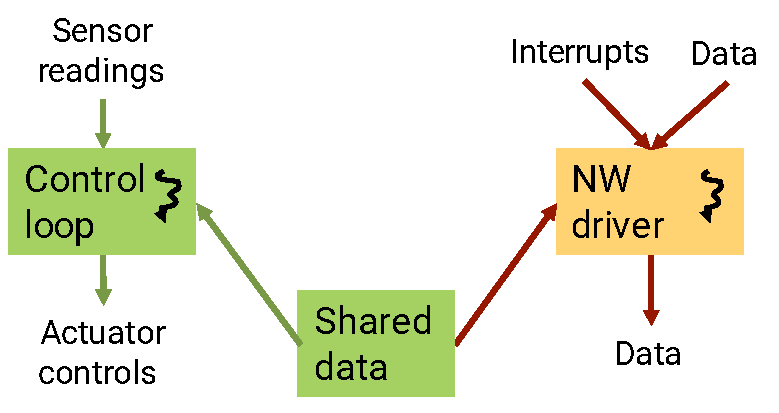
\includegraphics[width=0.55\textwidth]{mcs}
    \caption{Simplified example of a mixed-criticality system.}
    \label{f:mcs}
  \end{figure}

  Another big drawback of TSP is that interrupt latencies are
  inherently high. Take the example of \autoref{f:mcs}, which might
  represent a (highly simplified) autonomous vehicle. The critical
  component is a control loop, which executes once every 5\,ms to process
  sensor data and send commands to actuators. Its WCET, and therefore
  time slice, is 3\,ms. The vehicle also communicates with a ground
  station, which can update way points. Because the system operates on
  a 5\,ms period, this is the latency at which network interrupts can
  be processed, greatly limiting network throughput and generally
  responsiveness to external events.

  \SSSect{MCS support in seL4}

  The core challenge with MCS is that the OS must provide strong
  resource isolation, but TSP is overly simplistic (and thus inflexible). In
  terms of space resources, seL4 already has a
  flexible, powerful and provably secure model: object capabilities
  (see \autoref{s:caps}). MCS support extends this to time: access to
  the processor is now also controlled by capabilities.

  seL4's capabilities for processor time are called
  \emph{scheduling-context capabilities}. A component can only obtain
  processor time if it holds such a capability, and the amount of
  processor time it can use is encoded in the capability. This is
  analogous to the way access rights to spatial objects work.

  \begin{Chilli}
    In traditional seL4 (as in most L4 kernels before it) a thread had
    two main scheduling parameters: a \emph{priority} and a \emph{time
      slice}, which determine access to the processor. The priority
    determines when a thread can execute: it can run if there is no
    higher-priority thread runnable. The time slice determines how
    long the kernel will let the thread run before preempting it
    (unless it is preempted before by a higher priority thread becoming
    runnable). When the time slice is exhausted, the scheduler will
    again pick the highest-priority runnable thread (which may be the
    thread just preempted), with a round-robin policy used within
    priority levels.

    The  MCS version of seL4 replaces the time slice by a
    capability to a scheduling-context object, which performs a
    similar function, but in a more precise way that is the key to
    isolation: A scheduling context contains two main attributes. (1)
    a \emph{time budget}, which is similar to the old time slice, and
    limits the time for which a thread can execute until
    preempted. (2) a \emph{time period}, which determines how often the
    budget can be used: the thread will not get more time than one
    budget per period, preventing it from monopolising the CPU
    irrespective of its priority.
  \end{Chilli}

  Scheduling contexts support reasoning about the amount of time a thread
  can consume, and therefore, how much time is left. Specifically, they
  can be used to prevent a high-priority thread from monopolising the
  processor.

  \begin{Chilli}
    Applied to the above example, this means that we can give the
    (less critical) device driver a higher priority than the
    (critical) control component. This allows the driver to preempt
    the control, leading to high responsiveness. But the budget limit
    will stop the driver from monopolising the CPU.

    For example, we give the controller a budget of 3\,ms (its WCET)
    and a period of 5\,ms (corresponding to the frequency at which it
    operates). And we give the high-priority driver a small budget of
    3\,\(\mu\)s with a period of 10\,\(\mu\)s, meaning it can under no
    circumstances consume more than 30\% of total processor time, yet
    can execute frequently enough to ensure good
    responsiveness. Importantly we can guarantee that the control,
    which needs no more than 60\% of available processor time, is left
    with enough time to meet its deadline.
  \end{Chilli}

  By guaranteeing the critical deadline irrespective of the
  behaviour of the driver, we isolate the control from the untrusted
  driver, according to the core requirement of MCS. In particular,
  the driver need not be certified as safety-critical.

  seL4's time capability model addresses a number of other challenges
  of MCS, which go beyond the scope of this white paper, and we refer the
  interested reader to the peer-reviewed
  publication~\citep{Lyons_MAH_18}. Suffice to say that seL4 provides
  the most advanced and flexible MCS support of any OS suitable for
  critical systems.

  \Sect{Security is No Excuse for Poor Performance}\label{s:perf}

  Performance has always been the hallmark of L4 microkernels, and
  seL4 is no exception. We built seL4 for real-world use, and our aim
  was not to lose more than 10\% in IPC performance relative to the
  fastest kernels we had before. As it turns out, seL4 ended up beating the
  performance of those kernels.

  And it beats the performance of any other microkernel. This is a
  claim that is difficult to prove, as the competition generally holds
  their performance data close to their chest (for very good reason!)

  However, we make this performance claim, publicly, at every
  opportunity. If anyone disagrees they need to present evidence. We
  also know through a number of informal channels that IPC performance
  of other systems tends to range between 2 times slower than seL4
  to \emph{much} slower, typically around a factor of ten.

  The few independent performance comparisons certainly back our claim.

  \begin{Chilli}
    \citet{Mi_LYWC_19} compare the performance of three open-source
    systems, seL4, Fiasco.OC and Zircon. It finds that seL4 IPC costs
    are about 10--20\% above the hardware limit of kernel entry,
    address-space switch and kernel exit. Fiasco.OC is more than a factor
    of two slower than seL4 (close to three times the hardware limit),
    and Zircon is almost nine times slower than seL4.

    \citet{Gu_SCWKSC_16} compare the performance of CertiKOS to seL4,
    measuring 3,820 cycles for a round-trip IPC operation in CertiKOS
    compared to 1,830 in seL4, a factor of two. However, it turns out
    \code{sel4bench}, the seL4 benchmarking suite, had at the time a
    bug in dealing with timers on x86, resulting in exaggerated
    latencies. The correct
    \href{https://sel4.systems/About/Performance/}{seL4 performance
      figure} is around 720 cycles, or more than five times faster
    than CertiKOS. This is in the context of CertiKOS offering very
    limited functionality, and no capability-based security.
  \end{Chilli}

  \Sect{Real-World Deployment and Incremental Cyber
    Retrofit}\label{s:retrofit}

  \SSect{General considerations}

  When planning to \href{https://sel4.systems/Use/}{protect the
    security or safety of your system with seL4}, the first step
  should be to identify the critical assets you need to protect. The
  aim should be to minimise this part of your trusted computing base,
  and make it as modular as feasible, with each module becoming an
  seL4-protected CAmkES component.

  The other important preparation is to check
  \href{https://docs.sel4.systems/Hardware/}{availability}  and
  \href{https://docs.sel4.systems/projects/sel4/verified-configurations.html}{verification
    status} of seL4 on your platform. Obviously you will want a
  verified kernel, that's what seL4 is all about. However, even on
  platforms where the kernel is not verified, the fact that it shares
  much of its code with a verified platform will give you much higher
  assurance than with almost any other OS. But keep in mind that
  without verification the assurance is not what it can be. Also, you
  \href{https://sel4.systems/Foundation/Trademark/}{must not make any verification claim} if you are using a kernel
  that is not verified for your platform, or that is in any way
  modified.

  You furthermore will need to assess whether the
  \href{https://docs.sel4.systems/projects/available-user-components.html}{available
    user-level infrastructure} is sufficient for your purpose. If not,
  then this is where the community may help you. There are companies
  specialising in providing support for seL4 adoption. Also, if you
  develop any generally useful components yourself, you should
  seriously consider sharing them with the community under an
  appropriate open-source license. Those who give back will find it
  easier to get help from others.

  \SSect{Retrofitting existing systems}

  Most real-world deployments of seL4 will not run everything
  native. Typically, there are significant legacy components that would
  be expensive to port, because they are too big or rely on too many
  system services that are not presently supported by seL4. Also,
  frequently there would be little security or safety gain from
  running such legacy stacks natively.

  Using seL4's virtualisation capabilities is frequently the pragmatic
  way to proceed, \autoref{s:hyp} shows examples.

  The typical approach is what we call \emph{incremental
    cyber-retrofit}, a term coined by then DARPA program director John
  Launchbury. As \autoref{f:hacms} shows, this typically starts out by simply putting the whole existing
  software stack into a virtual machine running on seL4. Obviously
  this step buys nothing in terms of security and safety, it only adds
  (very small) overhead. Its significance is that it provides a
  baseline from where to start modularising.

  \begin{figure}[tb]
    \centering
    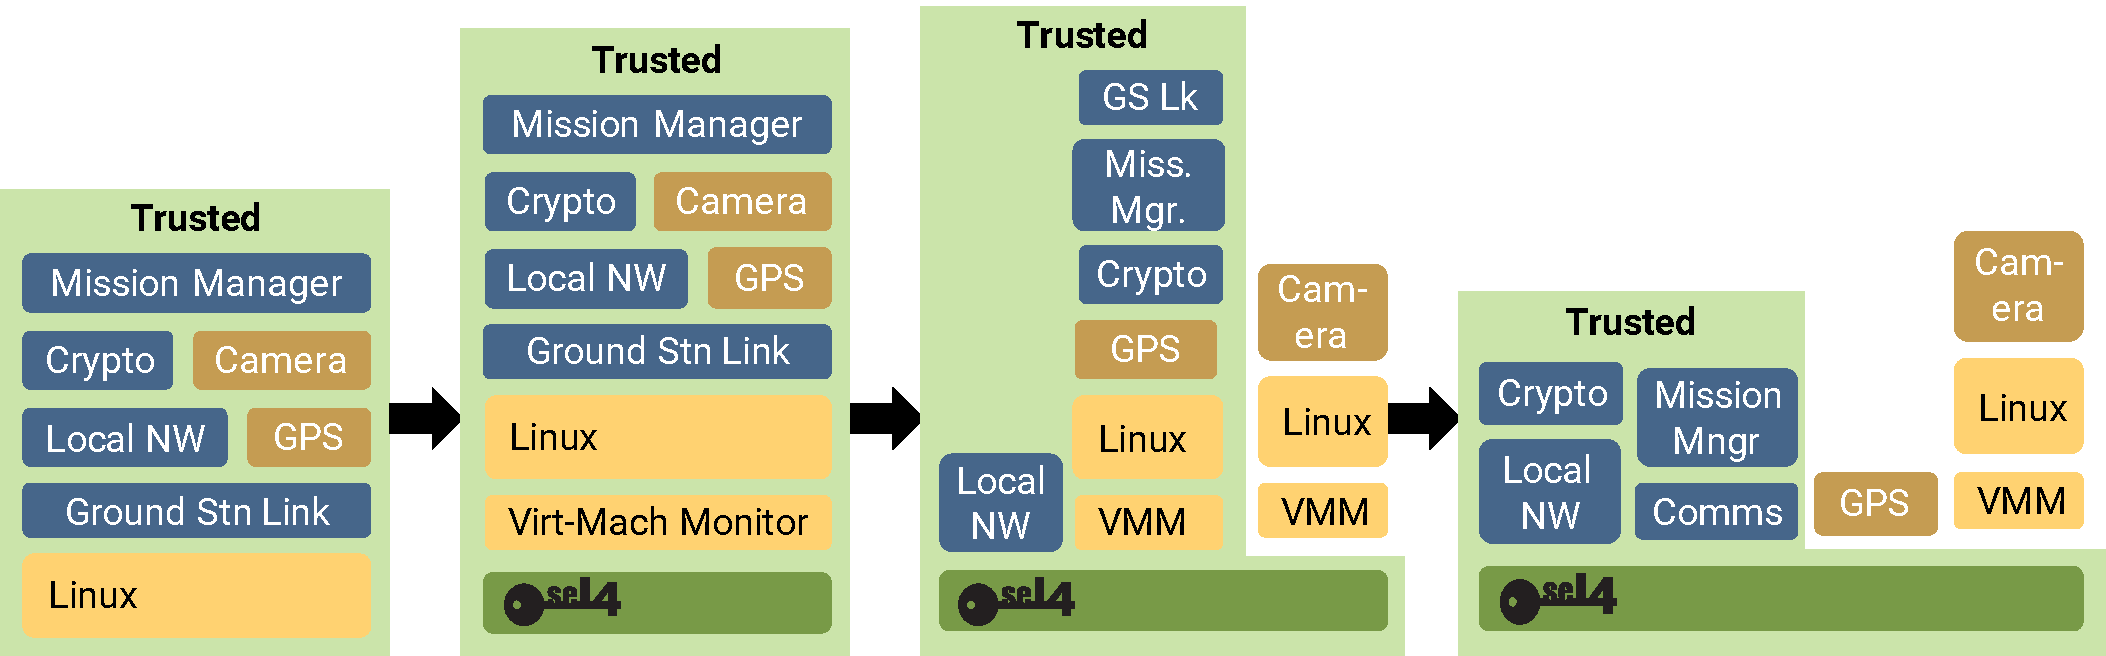
\includegraphics{hacms}
    \caption[Incremental cyber-retrofit on the ULB.]{Incremental
      cyber-retrofit of the Boeing ULB mission computer during the
      DARPA HACMS program.}
    \label{f:hacms}
  \end{figure}

  A great example is the work our \href{https://trustworthy.systems/projects/TS/SMACCM/}{HACMS project partners} did on cyber-retrofitting the Boeing
  ULB autonomous helicopter. The original system ran on Linux, and in
  a first step, the team put seL4 underneath.

  The next step broke out two components: The particularly untrusted
  camera software was moved to a second VM, also running Linux, with
  the two Linux VMs communicating via CAmkES channels. At the same
  time, the network stack was pulled out of the VM and converted to a
  native CAmkES component, also communicating with the main VM.

  The final step pulled all other critical modules, as well as the
  (untrusted) GPS software, into separate CAmkES components, removing
  the original main VM. The final system consisted of a number of
  CAmkES components running seL4-native code, and a single VM running
  just Linux and the camera software.

  The upshot was that while the initial system was readily hacked by
  the professional penetration testers hired by DARPA, the end state was highly
  resilient. The attackers could compromise the Linux system and do
  whatever they wanted with it, but were unable to break out and
  compromise any of the rest of the system. The team was confident
  enough to demonstrate an attack in-flight.

  \Sect{\label{s:concl}Conclusions}

  seL4 was the world's first OS kernel with a proof of implementation
  correctness (functional correctness). We then extended the
  verification down to the
  binary and up to security-enforcement properties, as explained in
  \autoref{s:proofs}.

  While by now there are other verified OS kernels, seL4 still defines
  the state of the art~\citep{Heiser:10y-blog}: It has the most
  comprehensive verification story, it is still the only
  capability-based OS that is verified, and it has the most advanced
  real-time support. And our ongoing research aims to ensure that
  seL4 will retain its position as the clear leader among security-
  and safety-oriented OSes, for example by pioneering systematic and
  principled prevention of information leakage through timing
  channels~\citep{Ge_YCH_19}.

  Besides this technological leadership, seL4 is in practical terms
  still far ahead of its successors: While we designed seL4 for
  real-world use from the beginning, almost all other verified OS
  kernels are academic toys, and far from real-world capable. In fact, we
  are only aware of one other (very recently) verified system that is
  practically deployable (although in far more limited scenarios).

  seL4's real-world readiness is a result of two aspects that drove
  the design: uncompromising performance focus, as highlighted in
  \autoref{s:perf}, and mechanisms that are designed to support the
  widest range of application scenarios and security policies, the
  latter enabled by capability-based access control
  (\autoref{s:caps}).

  Ten years of taking seL4 to the real-world, including
  cyber-retrofitting legacy systems (\autoref{s:retrofit}), has obviously
  helped us to refine and improve the system, but I'm proud to say that
  mild, incremental changes were sufficient. The one exception is the
  MCS support (\autoref{s:mcs}), which required a fairly significant change
  to the model and its implementation, but privileged management of
  time was the one thing we knowingly left in the to-do basket at
  the time of the original design~\citep{Heiser_Elphinstone_16}.

  This white paper has hopefully given you a reasonable idea of what
  seL4 is, what you can do with it, and, importantly, why you would
  want to use it. I hope this will help you become an active member of
  the seL4 community, including joining and participating in the
  \href{https://sel4.systems/Foundation}{seL4 Foundation}.

  I expect this document will keep evolving, and I am keen on
  feedback. But most of all, I'm keen to hear of your experience with
  deploying seL4.


  \Acks

  I gratefully acknowledge the feedback I received on earlier versions
  of this whitepaper, which helped improve it. The following members of TS commented on drafts:
  Curtis Millar,
  Gerwin Klein,
  Ihor Kuz,
  June Andronick,
  Liz Willer,
  Luke Mondy,
  Michael Norrish and
  Zoltan Kocsis.

  In addition I received comments from community members
  Ben Leslie and
  Davor Ocelic.

  Kim Pastor did a great job in creating the Foundation branding.
  \cleardoublepage
  \sloppy
  \bibliographystyle{plainnat}
  \bibliography{references}

\end{document}


%%% Local Variables:
%%% mode: latex
%%% TeX-master: t
%%% End:
